\documentclass[pdf,bluish,slideColor,colorBG]{prosper}
\hypersetup{pdfpagemode=FullScreen}
\usepackage{color}
\usepackage{graphicx}
\usepackage{amsfonts}
\usepackage{amsmath}
\def\baselinestretch{0.7}
\parindent 0.3in
\hyphenpenalty=10000
\tolerance=10000
\pagestyle{empty}

\def\Prob{{\rm Prob\;}}
\def\prob{{\rm \;Prob\;}}
\def\Var{{\rm Var}}        % Var
\def\Cov{{\rm Cov}}        % Cov

\DeclareSymbolFont{AMSb}{U}{msb}{m}{n}
\DeclareMathSymbol{\expect}{\mathalpha}{AMSb}{'105}

% bold math (use \bm{...})
\def\bm#1{\mathpalette\bmstyle{#1}}
\def\bmstyle#1#2{\mbox{\boldmath$#1#2$}}

\title{Comparative method and phylogenies}

\author{Joe Felsenstein}

\institution{Biology 550D}

\subtitle{\small \\ 3 November 2016}


\definecolor{orange}{rgb}{1.0,0.8,0.0}
\definecolor{Dandelion}{rgb}{0.8,0.4,0.3}
\definecolor{golden}{rgb}{1.0,0.75,0.2}
%\definecolor{golden}{rgb}{1.0,0.8,0.3}
\definecolor{purple}{rgb}{0.6,0.2,0.6}
\definecolor{darkblue}{rgb}{0.1,0.1,0.6}
\definecolor{yellow}{rgb}{1.0,1.0,0.0}
\definecolor{brightred}{rgb}{1.0,0.,0.0}
\definecolor{black}{rgb}{0.0,0.0,0.0}
\definecolor{white}{rgb}{1.0,1.0,1.0}
\definecolor{purple}{rgb}{0.8,0.0,0.8}

% sets backgroundcolor for whole document 
%\pagecolor{darkblue}
%\pagecolor{white}
% sets text color
%\color{yellow}
%\color{black}
% to change just a few words
% using \textcolor{color}{text}

\DeclareSymbolFont{AMSb}{U}{msb}{m}{n}
\DeclareMathSymbol{\expect}{\mathalpha}{AMSb}{'105}

\def\Prob{{\rm Prob\;}}
\def\prob{{\rm \;Prob\;}}
\def\Var{{\rm Var}}        % Var
\def\Cov{{\rm Cov}}        % Cov

\begin{document}

% OUTLINE ALL TALKS
% Brownian motion approximation
% Edwards and Cavalli-Sforza
% me, 1968/1973
% Lande, 1976 
% REML trees with Brownian motion
% Pruning
% Inferring the covariances?
% incl. Grafen (and/or PGLS)
% The determinant result (make sure Jacobian included)
% Some kind of simulation with finite number of loci w/mutation
% 
% Source of covariation (VA, selective)
% 
% Ornstein-Uhlenbeck (Marguerite?)
% Chasing a peak
% Go where peak goes
% Smoothing caused by this
% Equilibrium covariances
% Tree covariation
% 
% Morphometrics
% Bookstein
% Alignment
% Rotation and optimization (and approximations)
% Need for special models

% Threshold models
% Sewall Wright( and guinea pig)
% 


\maketitle

{
\parindent=0in

\begin{slide}[Replace]{A simple case to show effects of phylogeny}
\bigskip

\centerline{\includegraphics[height=2in]{fig25-2.ydraw}}

\end{slide}

\begin{slide}[Replace]{Two uncorrelated characters evolving on that tree}

\centerline{\includegraphics[height=3in]{fig25-3a.ydraw}}

\end{slide}

\begin{slide}[Replace]{Identifying the two clades}

\centerline{\includegraphics[height=3in]{fig25-3b.ydraw}}

\end{slide}

\begin{slide}[Replace]{A tree on which we are to observe two characters}
\bigskip

\centerline{\includegraphics[height=2.4in]{fig25-4.ydraw}}

\end{slide}

\begin{slide}[Replace]{Contrasts on that tree}

\[
\begin{array}{c c c c c c c c c c c l}
 & & & & & & & & & & & \multicolumn{1}{c}{$\rm Variance$} \\
 & & & & & & & & & & & \multicolumn{1}{c}{$\rm proportional$}\\
\multicolumn{7}{c}{\rm Contrast} & & & & & \multicolumn{1}{c}{$\rm to$} \\
 & & & & & & & & & & & \\
\mathsf{y_1} & \mathsf{=} & \mathsf{x_a} & \mathsf{-} & \mathsf{x_b} & & & & & & & \mathsf{~~~0.4}  \\
 & & & & & & & & & & & \\ 
\mathsf{y_2} & \mathsf{=} &\mathsf{\frac{1}{4}\;x_a} & \mathsf{+} & \mathsf{\frac{3}{4}\;x_b} & \mathsf{-} & \mathsf{x_c} & & & & & \mathsf{~~~0.975} \\ & & & & & & & & & & & \\ 
\mathsf{y_3} & \mathsf{=} & & & & & & & \mathsf{x_d} & \mathsf{-} & \mathsf{x_e} & \mathsf{~~~0.2} \\
 & & & & & & & & & & & \\ 
\mathsf{y_4} & \mathsf{=} & \mathsf{\frac{1}{6}\;x_a} & \mathsf{+} & \mathsf{\frac{1}{2}\;x_b} & \mathsf{+} & \mathsf{\frac{1}{3}\;x_c} & \mathsf{-} & \mathsf{\frac{1}{2}\;x_d} & \mathsf{-}  & \mathsf{\frac{1}{2}\;x_e} & \mathsf{~~~1.11666}
\end{array}
\]

\end{slide}

\begin{slide}[Replace]{Joint distribution for multiple species, characters}
\bigskip

\centerline{\includegraphics[width=3in]{multibrownian.idraw}}
\bigskip

Consider change of two characters, each assessed in a different species.  Say
character $~\mathsf{x}~$ and character $~\mathsf{y}$, the first measured
in species 2, the second in species 3.   The result will give us the pattern
for any two characters measured in any two species.
\bigskip

\end{slide}

\begin{slide}[Replace]{Seeing that covariances are zero in different branches ... }
\bigskip

\[
\mathsf{\Cov[ \Delta x_1 + \Delta x_2, \ \ \Delta y_1 + \Delta y_3]}
\]

Given that changes in different branches are independent (whether changes of
the same character or of different characters), the only nonzero covariance
is between $~\mathsf{\Delta x_1}~$ and $~\mathsf{\Delta y_1}.$

\[
\mathsf{\Cov[ \Delta x_1 + \Delta x_2, \ \ \Delta y_1 + \Delta y_3]}
\]

\[
\mathsf{ \ = \ \Cov[ \Delta x_1, \ \: \Delta y_1]}
\]

So the covariance of different characters in different species is the
product of the shared evolution to their common ancestor by the
(infinitesimal) covariance of the character change per unit branch length.

\end{slide}


\begin{slide}[Replace]{Joint distribution for many species, many characters}
\bigskip

The upshot is that if $~\mathsf{x_{ik}}~$ is character $~\mathsf{k}~$ in species$~\mathsf{i}$, and $~\mathsf{x_{j\ell}}~$ is character
$~\mathsf{\ell}~$ in species $~\mathsf{j}$, the covariance between them is
\[
\mathsf{Cov [x_{ik}, x_{j\ell}] \ = \ t_{ij}\;v_{k\ell}}
\]
where $~\mathsf{t_{ij}}~$ is the time (branch length) to the latest common ancestor of
species $~\mathsf{i}~$ and species $~\mathsf{j}$. $\mathsf{\bf V}~$ is the covariance matrix of evolutionary
change for the characters.

\end{slide}

\begin{slide}[Replace]{Covariances of species on the tree}
\bigskip

{\ptsize{8}
\[
\hspace*{0in}\hspace{-0.34in}\left[\hspace{-0.1in}
\begin{array}{c c c c c c c c c c c c c}
\multicolumn{3}{c}{\mathsf{v_1+v_8+v_9}} & \mathsf{v_8+v_9} & & \mathsf{v_9} & & \mathsf{0} & & \mathsf{0} & & \mathsf{0} & \mathsf{0} \\
& \mathsf{v_8+v_9} & \multicolumn{3}{c}{\mathsf{v_2+v_8+v_9}} & \mathsf{v_9} & & \mathsf{0} & & \mathsf{0} & & \mathsf{0} & \mathsf{0}\\
& \mathsf{v_9}     & & \mathsf{v_9} & \multicolumn{3}{c}{\mathsf{v_3+v_9}} & \mathsf{0} & & \mathsf{0} & & \mathsf{0} & \mathsf{0} \\
& \mathsf{0}       & & \mathsf{0} & & \mathsf{0} & \multicolumn{3}{c}{\mathsf{v_4+v_{12}}} & \mathsf{v_{12}} & & \mathsf{v_{12}} & \mathsf{v_{12}} \\
& \mathsf{0}       & & \mathsf{0} & & \mathsf{0} & & \mathsf{v_{12}} & \multicolumn{3}{c}{\mathsf{v_5+v_{11}+v_{12}}} & \mathsf{v_{11}+v_{12}} & \mathsf{v_{11}+v_{12}} \\
& \mathsf{0}       & & \mathsf{0} & & \mathsf{0} & & \mathsf{v_{12}} & & \mathsf{v_{11}+v_{12}} & \multicolumn{2}{c}{\mathsf{v_6+v_{10}+v_{11}+v_{12}}} & \mathsf{v_{10}+v_{11}+v_{12}} \\
& \mathsf{0} & & \mathsf{0} & & \mathsf{0} & & \mathsf{v_{12}} & & \mathsf{v_{11}+v_{12}} & \multicolumn{2}{c}{\mathsf{v_{10}+v_{11}+v_{12}}} & \mathsf{v_7+v_{10}+v_{11}+v_{12}} \\
\end{array}\hspace{-0.05in}\right]
\]
}

\end{slide}

\begin{slide}[Replace]{Covariances are of form }
\bigskip

{\ptsize{10}
\[
\left[
\begin{array}{c  c c | c c c c}
\multicolumn{1}{c|}{\mathsf{a}} & \multicolumn{1}{c|}{\mathsf{b}} & \mathsf{c} & \mathsf{0} & \mathsf{0} & \mathsf{0} & \mathsf{0} \\
\cline{1-2}
\multicolumn{1}{c|}{\mathsf{b}} & \multicolumn{1}{c|}{\mathsf{d}} & \mathsf{c} & \mathsf{0} & \mathsf{0} & \mathsf{0} & \mathsf{0} \\
\cline{1-3}
\mathsf{c} & \multicolumn{1}{c|}{\mathsf{c}} & \mathsf{e} & \mathsf{0} & \mathsf{0} & \mathsf{0} & \mathsf{0} \\
\hline
\mathsf{0} & \mathsf{0} & \mathsf{0} & \multicolumn{1}{c|}{\mathsf{f}} & \mathsf{g} & \mathsf{g} & \mathsf{g} \\
\cline{4-7}
\mathsf{0} & \mathsf{0} & \mathsf{0} & \multicolumn{1}{c|}{\mathsf{g}} & \multicolumn{1}{c|}{\mathsf{h}} & \mathsf{i} & \mathsf{i} \\
\cline{5-7}
\mathsf{0} & \mathsf{0} & \mathsf{0} & \multicolumn{1}{c|}{\mathsf{g}} & \multicolumn{1}{c|}{\mathsf{i}} & \multicolumn{1}{c|}{\mathsf{j}} & \mathsf{k} \\
\cline{6-7}
\mathsf{0} & \mathsf{0} & \mathsf{0} & \multicolumn{1}{c|}{\mathsf{g}} & \multicolumn{1}{c|}{\mathsf{i}} & \multicolumn{1}{c|}{\mathsf{k}} & \mathsf{l} \\
\end{array}
\right]
\]
}

\end{slide}

\begin{slide}[Replace]{ ``Pruning'' a tree in the Brownian motion case}
\bigskip

One can take two neighboring tips, and consider their difference $\ \mathsf{x_1 -
x_2\ }$ as well as a weighted average $\ \mathsf{a x_1 + (1-a) x_2}$.  Using
  weights $\mathsf{a\, :\, 1-a \ = \  1/v_1\, :\, 1 /v_2}$, the weighted average is
independent of the difference, and the difference is also independent of the
rest of the tree.
\bigskip

In fact, this weighted average behaves like a tip:  Its covariances with
the other species are the same as those of $\mathsf{x_1}$ and $\mathsf{x_2}$.
It acts just as if the tree were pruned, cutting off species 1 and 2, leaving
a single species whose variance is a bit bigger.
\bigskip

\[
\mathsf{\Var[a x_1 + (1-a) x_2] \ = \  v_8 + v_9 + \frac{v_1 v_2}{v_1 + v_2}}
\]

so in effect, a small extra amount of branch length is added.

\end{slide}

\begin{slide}[Replace]{ ``Pruning'' a tree in the Brownian motion case}

\centerline{\includegraphics[height=2.2in]{fig23-3.ydraw}}

\medskip
(True in the sense that the log-likelihoods -- which are a bit different
than the usual likelihoods -- add up, since the likelihoods multiply).

\end{slide}

\begin{slide}[Replace]{Contrasts for the 20-species two-clade example}

\centerline{\includegraphics[height=3in]{fig25-5.ydraw}}

\end{slide}

\begin{slide}[Replace]{The algebra}

If $\bf{T}$ is the covariances of $~\mathsf{n}~$ tips on the tree, and $\bf{V}$ is the (unknown) covariances of the Brownian motion of the $~\mathsf{p}~$ characters, the log-likelihood of
a set of characters (stacked as a vector) $\bf{x}$ is
\[
\ln L \ = \ - (np/2) \ln (2\pi) - (1/2) \ln |{\bf T}\otimes{\bf V}| - (1/2) ({\bf x-\mu})^t ({\bf T}\otimes{\bf V})^{-1} ({\bf x-\mu})
\]
If ${\bf C}$ is an $~\mathsf{(n-1) \times n}~$ set of contrasts, each
orthogonal to the grand mean, such that ${\bf CTC}^t$ is an $~\mathsf{n-1}$-dimensional identity matrix, then taking the density of the transformed data
{\bf y} = {\bf C} {\bf x}, this has expectation vector {\bf 0}:
\[
\ln L \ = \ K - (1/2) \ln |{\bf I}_{n-1}\otimes{\bf V}| - (1/2) {\bf y}^t ({\bf I}_{(n-1)}\otimes{\bf V})^{-1} {\bf y}
\]
(where $K$ collects the constant stuff, including the $\mathsf{\ln(v_1+v_2)}$) Jacobian term.

\end{slide}

\begin{slide}[Replace]{ ... simplifying ... }

  This can also be expressed as
\[
\ln L \ = \ K - ((n-1)/2) \ln |{\bf V}| - (1/2) {\rm tr} \left({\bf S} {\bf V})^{-1} \right)
\]
where
\[
{\bf S} \ = \ \sum\limits_i {\bf y}^{(i)} \left({\bf y}^{(i)}\right)^t
\]
is the $~\mathsf{p \times p}~$ sum of squares matrix of characters across contrasts. 

Inferring the Brownian motion phylogenetic covariances by maximum likelihood
we find that
\[
\widehat{\bf V} \ = \ {\bf S} / (n-1)
\]
which leads to
\[
\ln L \ = \ K' \ - \ ((n-1)/2) \ln |\widehat{\bf V}|
\]
\end{slide}

\begin{slide}[Replace]{The case of observing ancestors}
\medskip

\centerline{\includegraphics[height=1.3in]{lineage.idraw}}

This works out as one might hope.  Computing the contrasts, they turn out to be
simply

\[
\mathsf{\frac{x_1-x_0}{\sqrt{v_1}}, \ \  \ 
\frac{x_2-x_1}{\sqrt{v_2}}, \ \  \ 
\frac{x_3-x_2}{\sqrt{v_3}}, \ \  \ 
\frac{x_4-x_3}{\sqrt{v_4}}}
\]
\medskip

which are obviously independent.
\medskip

In the case where a finite sample is taken at each time, and there is
within-species phenotypic variation, matters are more complicated but a
comparative methods analysis allowing for sampling error works.
\bigskip

\end{slide}

\begin{slide}[Replace]{A research program? }
\bigskip

What we could imagine doing is:

\begin{itemize}
\item We might hope to infer additive genetic covariances by doing quantitive
genetics breeding experiments to infer them from covariances among relatives,
perhaps even in multiple species.
\item Infer the covariances of the changes along the phylogeny.
\item From them, back-calculate the selective covariances.
\item The genetic covariances may also be inferrable from differences between
nearby tips on the tree if we do not have breeding experiments.
\item There is little or no hope of inferring ``selective correlations''
more directly without a complete understanding of the functional ecology.
\end{itemize}

\end{slide}

\begin{slide}[Replace]{An example: Riek and Geiser, 2013 }

Alexander Riek and Fritz Geiser. 2013.  Allometry of thermal variables in mammals: consequences of body size and phylogeny. {\it Biological Reviews} {\bf 88 (3):} 564-572.

\vspace{-0.55in}
\begin{tabular}{c c}
\includegraphics[width=2.2in]{tips.ps} &
\includegraphics[width=2.2in]{contrasts.ps} \\[-0.45in]
body temperature vs. log(body size)  & contrasts vs. contrasts \\
($P$ for slope $\neq 0$ is $0.000375$)  &  ($P$ for slope $\neq 0$ is $0.116$) 
\end{tabular}

\end{slide}

\begin{slide}[Replace]{A simulated example}
\medskip

Using an ordinary regression with the species as points, we see a
significant relationship between brain weight and body weight:
\medskip

\centerline{\includegraphics[width=3in]{points.idraw}}
\bigskip

It looks as if we have 16 independent data points and a positive correlation between
brain weight and body weight across species.

\end{slide}

\begin{slide}[Replace]{But the points are not independent}
\bigskip

They evolved on a phylogeny.  More closely related points are similar.

\centerline{\includegraphics[width=3in]{plotfile.idraw}}

\end{slide}

\begin{slide}[Replace]{Using contrasts on the phylogeny ... }
\bigskip

\phantom{They evolved on a phylogeny.  More closely related points are similar.}

\centerline{\includegraphics[width=3in]{plotfilec.idraw}}

\end{slide}

\begin{slide}[Replace]{Is evolution of brain and body weight correlated? }
\bigskip

\centerline{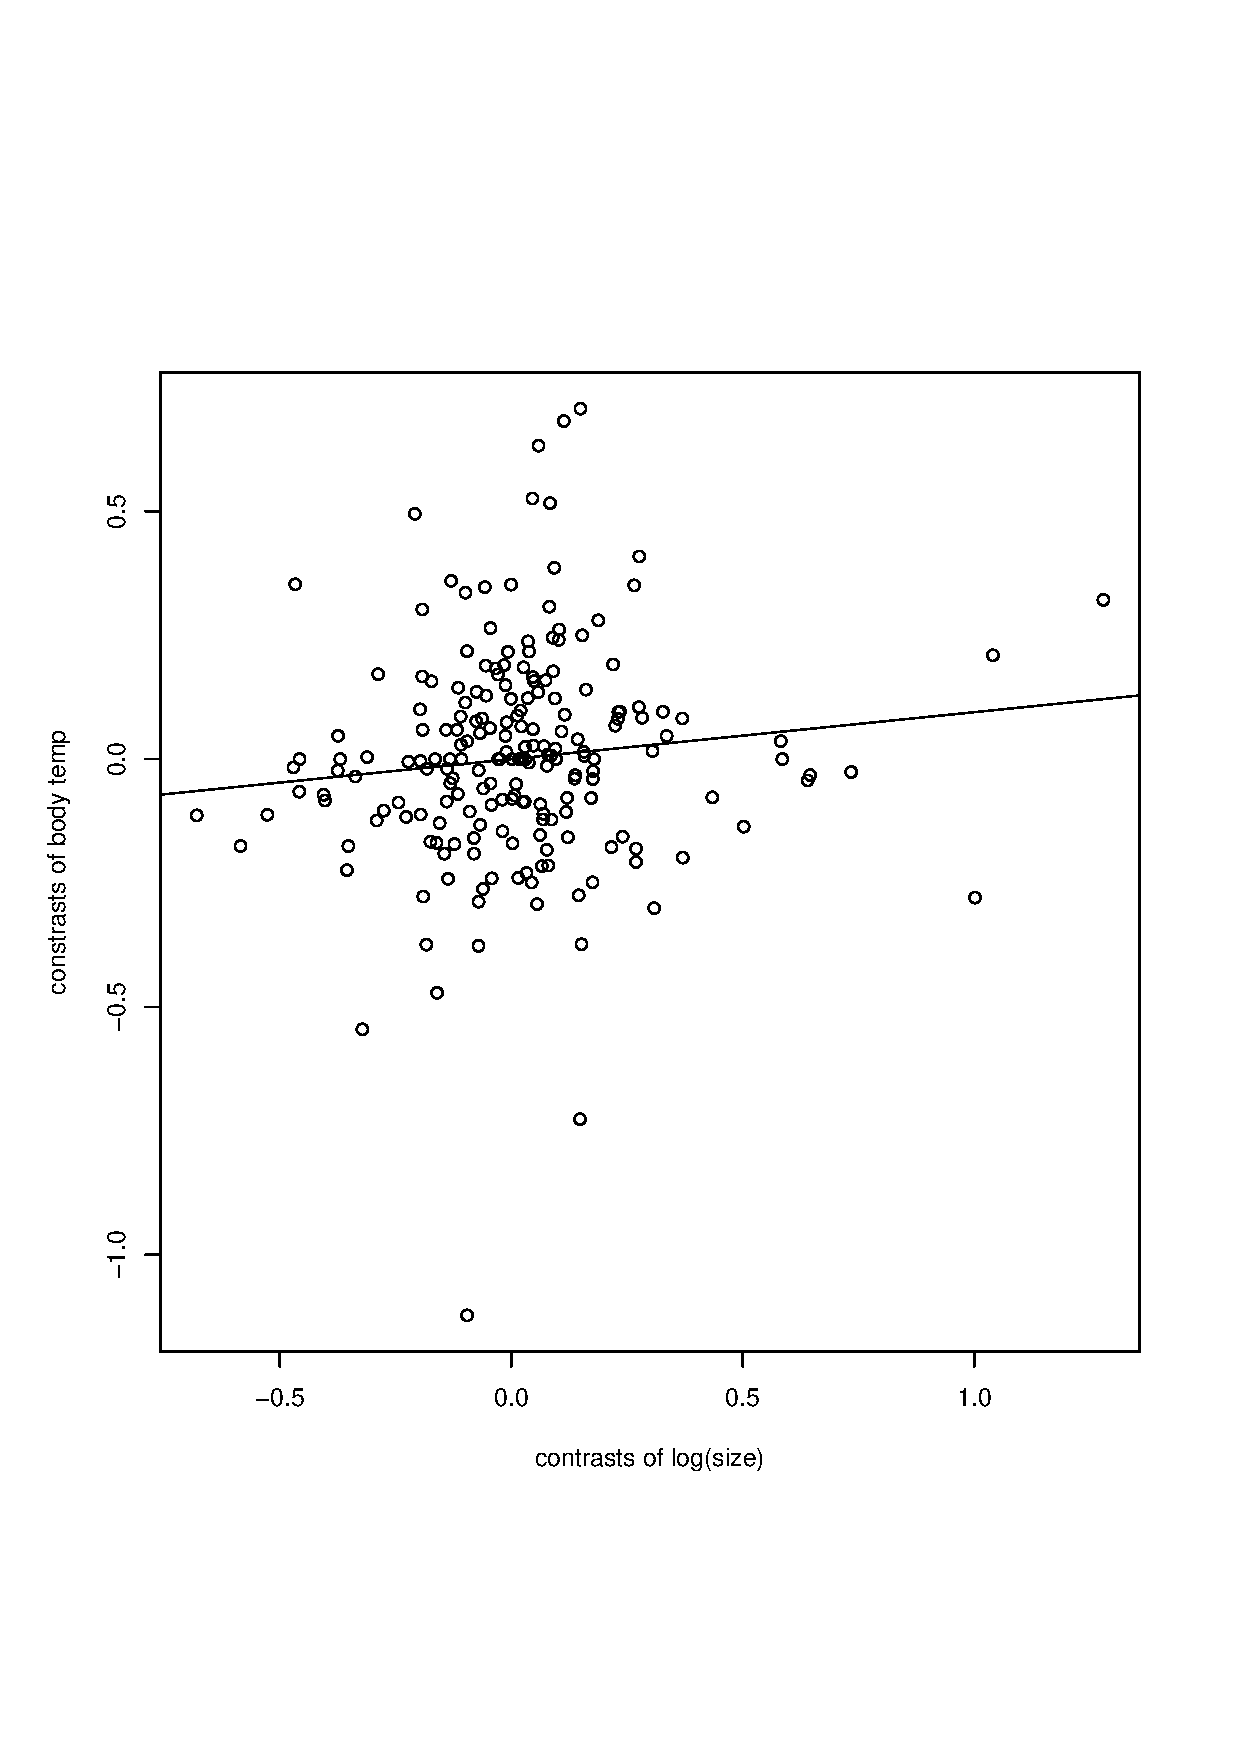
\includegraphics[width=3in]{contrasts.idraw}}
\bigskip

Using the contrasts method we see no significant relationship.

\end{slide}

\begin{slide}[Replace]{When the tree is noisy: Propagating bootstrap sampling}

\centerline{\includegraphics[width=4in]{propagatebs1a.ydraw}}

\end{slide}

\begin{slide}[Replace]{Propagating bootstrap sampling}

\centerline{\includegraphics[width=4in]{propagatebs1b.ydraw}}

\end{slide}

\begin{slide}[Replace]{Propagating bootstrap sampling}

\centerline{\includegraphics[width=4in]{propagatebs1c.ydraw}}

\end{slide}

\begin{slide}[Replace]{Propagating bootstrap sampling}

\centerline{\includegraphics[width=4in]{propagatebs1d.ydraw}}

\end{slide}

\begin{slide}[Replace]{Propagating bootstrap sampling}

\centerline{\includegraphics[width=4in]{propagatebs2.ydraw}}

\end{slide}

\begin{slide}[Replace]{Propagating bootstrap sampling}

\centerline{\includegraphics[width=4in]{propagatebs3.ydraw}}

\end{slide}

\begin{slide}[Replace]{Propagating bootstrap sampling}

\centerline{\includegraphics[width=4in]{propagatebs100.ydraw}}

\end{slide}

\begin{slide}[Replace]{A Bayesian model}

\centerline{\includegraphics[width=4in]{propagatebayes1a.ydraw}}

\end{slide}

\begin{slide}[Replace]{A Bayesian model}

\centerline{\includegraphics[width=4in]{propagatebayes1b.ydraw}}

\end{slide}

\begin{slide}[Replace]{A Bayesian model}

\centerline{\includegraphics[width=4in]{propagatebayes1c.ydraw}}

\end{slide}

\begin{slide}[Replace]{Bayesian MCMC}

\centerline{\includegraphics[width=4in]{propagatebayes1d.ydraw}}

\end{slide}

\begin{slide}[Replace]{Bayesian MCMC}

\centerline{\includegraphics[width=4in]{propagatebayes2.ydraw}}

\end{slide}

\begin{slide}[Replace]{Bayesian MCMC}

\centerline{\includegraphics[width=4in]{propagatebayes3.ydraw}}

\end{slide}

\begin{slide}[Replace]{Bayesian MCMC}

\centerline{\includegraphics[width=4in]{propagatebayes4.ydraw}}

\end{slide}

\overlays{6}{
\begin{slide}[Replace]{Some complications}

\begin{itemstep}
\item (As noted above) dealing with uncertainty about the phylogeny
\item Small sample size from species means their species means are
uncertain.  Must use a model with another level of variation -- within-species
phenotypic variation (Ricklefs and Starck, 1996; Ives et al., 2007; 
Felsenstein, 2008)
\item Rate of change of morphological characters need not be constant on the
molecular tree branch lengths.
\item Note -- regressions involving contrasts should assume that they all have
expectation zero. (They do because we don't know which lineage at a fork will
move further to the right on the phenotype scale).
\item How to infer the effect of an environmental variable when only its present-day values are known but not its values when the past changes were occurring?
(note: regressing on the present-day values is generally {\bf wrong}, see
paper by Hansen and Bartoszek, {\it Systematic Biology}, 2012).
\item Might be able to assume environment does Brownian motion and infer
covariances.  But this itself is a somewhat arbitrary assumption.
\end{itemstep}

\end{slide}
}

\overlays{6}{
\begin{slide}[Replace]{Poor inference of covariation -- what to do with that?}
\bigskip

 
\begin{itemstep}
\item Covariances are hard to infer with only (say) 50 species sampled
\item ... particularly if they samples are not independent but on a tree
\item ... particularly if the quantitative characters are thresholded
\item How do we propagate the resulting uncertainty when biologists want
``fly on the wall'' certainty?
\item Expanding to more species may put the model at risk
\item Expanding to more characters just adds new parameters to estimate
\end{itemstep}

\end{slide}
}
 
\begin{slide}[Replace]{References for phylogenetic comparative methods}

Felsenstein, J. 1985. Phylogenies and the
comparative method. {\it American Naturalist} {\bf 125:} 1--5.
\textcolor{purple}{\bf [Introduces the contrasts method]}
\medskip

Felsenstein, J. 1988. Phylogenies and quantitative characters. {\it Annual 
Review of Ecology and Systematics} \textcolor{purple}{\bf [Suggests using
bootstrapping to correct comparative methods for uncertainty about the
phylogeny} {\bf 19:} 445--471.
\medskip

Harvey, P. H. and M. D. Pagel. 1991. {\it The Comparative Method in
Evolutionary Biology.} Oxford University Press, Oxford. 
\textcolor{purple}{\bf [The major book introducing statistical phylogenetic comparative methods]}
\medskip

Grafen, A. 1989. The phylogenetic regression.  {\it Philosophical Transactions 
of the Royal Society of London, Series B} {\bf 326:} 119--157.  \textcolor{purple}{\bf [Using generalized least squares to evaluate the likelihood for
Brownian Motion phylogenies and do comparative methods analysis, without the
contrasts methods. In the simplest case, is exactly equivalent to the contrasts
method.  Discusses ways of coping with unresolved parts of the
phylogeny and with varying evolutionary rates.]}
\medskip

\end{slide}

\begin{slide}[Replace]{References, continued}

Ricklefs, R. E. and J. M. Starck. 1996.  Applications of phylogenetically
independent contrasts: A mixed progress report. {\it Oikos} {\bf 77:} 167--172.
\textcolor{purple}{\bf [Pointing put that small sample size within species is
a problem for comparative methods]}
\medskip

Ives, A. R., P. E. Midford, and T. Garland. 2007. Within-species
variation and measurement error in phylogenetic
comparative methods. {\it Systematic Biology} {\bf 56:} 252-270.
\textcolor{purple}{\bf [Taking small sample size into account when we
know the within-species phenotypic covariances]}
\medskip

Hansen, T. F., and K. Bartoszek.  2012. Interpreting the evolutionary regression: the interplay between observational and biological errors in phylogenetic comparative studies.  {\it Systematic Biology} {\bf 61(3):} 413 –- 425.
\medskip

Felsenstein, J. 2008 Comparative methods with
sampling error and within-species variation: contrasts
revisited and revised. {\it American Naturalist} {\bf 171:} 713--725.
\textcolor{purple}{\bf [Inferring both between=species evolutionary
covariances and within-species phenotypic variation]}
\medskip

Felsenstein, J.  2004.  {\it Inferring Phylogenies.}  Sinauer Associates,
Sunderland, Massachusetts. \textcolor{purple}{\bf Mentions this model and
also sample size issues in contrasts method.}
\medskip

\end{slide}
}
\end{document}

